\documentclass[a4paper,11pt]{article}

% --------------------------------------
% ENCODAGE ET LANGUE
% --------------------------------------
\usepackage[utf8]{inputenc}     % Encodage UTF-8
\usepackage[T1]{fontenc}        % Codage des caractères
\usepackage[french]{babel}      % Langue du document : français

% --------------------------------------
% MISE EN PAGE
% --------------------------------------
\usepackage{geometry}           % Gestion de la géométrie de page
\geometry{a4paper, margin=2.5cm}

% --------------------------------------
% TYPOGRAPHIE ET STYLE
% --------------------------------------
\usepackage{microtype}          % Amélioration de la justification du texte
\usepackage{lmodern}
\usepackage{enumitem}           % Listes personnalisées
\usepackage{caption}            % Gestion fine des légendes
\usepackage{graphicx}           % Insertion d’images

% --------------------------------------
% MATHÉMATIQUES
% --------------------------------------
\usepackage{amsmath}            % Formules mathématiques
\usepackage{amssymb}            % Symboles mathématiques

% --------------------------------------
% ALGORITHMIQUE
% --------------------------------------
\usepackage{algorithm}          % Environnement pour les algorithmes
\usepackage{algpseudocode}      % Style pseudo-code

% --------------------------------------
% HYPERLIENS ET NAVIGATION
% --------------------------------------
\usepackage[hidelinks]{hyperref} % Liens cliquables (TOC, références)
\usepackage{cleveref}            % Références intelligentes : \cref

% --------------------------------------
% EN-TÊTE ET PIED DE PAGE
% --------------------------------------
\usepackage{fancyhdr}
\pagestyle{fancy}
\fancyhf{} % Réinitialise tout

% En-tête
\fancyhead[R]{MIASHS - Outils financiers}

% Pied de page
\fancyfoot[L]{Boya | Seddouki | Layada }
\fancyfoot[C]{Université de Clermont Auvergne}
\fancyfoot[R]{\thepage}

\renewcommand{\headrulewidth}{0.4pt} % Ligne sous l’en-tête
\renewcommand{\footrulewidth}{0.4pt} % Ligne au-dessus du pied de page

% --------------------------------------
% DÉBUT DU DOCUMENT
% --------------------------------------

\begin{document}

\begin{center}
	\Huge{Projet De Mathématiques Financières}\\[0.5cm]
	\Large{Erkin Tunc Boya | Rania Seddouki |  Nasrallah Layada }\\ [0.2cm]
	\Large{Groupe 13} \\[0.2cm]
	\Large{Mars - Avril 2025}
\end{center}

\tableofcontents
\section{Introduction}

\subsection{Contexte du projet}

Dans le cadre de ce projet de mathématiques financières, nous nous intéressons à l’optimisation d’une stratégie d’investissement sur une période de temps donnée. Un investisseur dispose d’un capital initial qu’il peut placer de deux manières :
\begin{itemize}
	\item à un taux d’intérêt de base constant appliqué à chaque période individuelle ;
	\item via des produits financiers spécifiques offrant des rendements plus intéressants, mais sur des intervalles plus longs.
\end{itemize}

Ces options sont limitées dans le temps et ne sont pas toujours disponibles simultanément. Cela soulève naturellement la question du meilleur enchaînement possible de placements pour maximiser le capital final.

\subsection{Objectif et approche adoptée}

L’objectif principal est de déterminer une politique d’investissement optimale permettant de maximiser le capital final à l’issue de la période d’étude.

Pour résoudre ce problème, nous utilisons :
\begin{itemize}
	\item une \textbf{modélisation mathématique} du problème sous forme d’un graphe orienté représentant les différentes possibilités de placements ;
	\item une \textbf{approche algorithmique} basée sur la programmation dynamique, évitant l’énumération exhaustive de toutes les possibilités, qui serait inefficace dès que l’horizon d’investissement devient important.
\end{itemize}

Dans la suite du rapport, nous allons présenter le modèle, illustrer son fonctionnement à travers un exemple concret, détailler les étapes algorithmiques et conclure par une analyse des résultats obtenus.


    

\section{Modélisation mathématique}
\subsection{Hypothèses et notations}

L’horizon d’étude est une période discrète notée $T = [0, n]$, divisée en $n$ unités de temps. Un investisseur peut placer son capital de deux manières :
\begin{itemize}
	\item \textbf{Placement de base} : À chaque période $[t, t+1]$, un taux d’intérêt fixe $\tau_0$ est appliqué. Il est disponible en continu sur toute la période $T$.
	\item \textbf{Placements spécifiques} : On dispose de $m$ opportunités de placement $P_k = (d_k, f_k, \tau_k)$ avec :
	      \begin{itemize}
	      	\item $d_k$ : date de début du placement $k$ ;
	      	\item $f_k$ : date de fin du placement $k$ ;
	      	\item $\tau_k$ : taux d’intérêt applicable sur l’intervalle $[d_k, f_k]$.
	      \end{itemize}
\end{itemize}

Chaque placement $P_k$ ne peut être utilisé qu’une seule fois et uniquement sur l’intervalle $[d_k, f_k]$.
    

\subsection{Représentation par un graphe orienté}

Pour modéliser ce problème, nous utilisons un graphe orienté noté $D = (V, A)$ :

\begin{itemize}
	\item L’ensemble des \textbf{sommets} $V$ correspond aux dates $t \in \{0, 1, ..., n\}$.
	\item L’ensemble des \textbf{arcs} $A$ contient deux types de transitions :
	      \begin{itemize}
	      	\item Les arcs de base $(t, t+1)$ avec un coefficient $c(t, t+1) = 1 + \tau_0$ ;
	      	\item Les arcs spécifiques $(d_k, f_k)$ correspondant aux produits d’investissement, avec $c(d_k, f_k) = 1 + \tau_k$.
	      \end{itemize}
\end{itemize}

Chaque chemin dans ce graphe représente une stratégie d’investissement possible.


\subsection{Chemins et stratégie de placement}

Un \textbf{chemin} $P$ du sommet $0$ au sommet $n$ dans le graphe $D$ représente une séquence de décisions d’investissement. À chaque étape, le capital est multiplié par le coefficient de l’arc emprunté.

On définit :
\[
	C(P) = \prod_{a \in P} c(a)
\]
\indent comme le \textbf{coefficient multiplicatif total} associé à un chemin $P$.

L’objectif est de déterminer le chemin $P^*$ tel que :
\[
	C(P^*) = \max_{P \in \mathcal{P}(0, n)} C(P)
\]

où $\mathcal{P}(0, n)$ est l’ensemble des chemins allant de 0 à $n$ dans le graphe.

Pour cela, on introduit une fonction de programmation dynamique :
\[
	\text{Coef}(t) = \max_{P \in \mathcal{P}(0, t)} C(P)
\]
avec l’initialisation $\text{Coef}(0) = 1$. Cette fonction permet de calculer de manière séquentielle la valeur maximale atteignable à chaque date $t$.

\subsection{Cardinalité des chemins dans le graphe}

Le nombre de chemins possibles de 0 à $n$ dépend de la structure du graphe $D$.

\paragraph{Cas général (avec seulement les arcs $(t, t+1)$)} 
Si l’on ne considère que les placements de base (un seul arc $(t, t+1)$ entre deux dates consécutives), alors il n’existe qu’un seul chemin possible de 0 à $n$.

\paragraph{Cas complet (tous les arcs $(t', t)$ possibles pour $t' < t$)} 
Si le graphe contient tous les arcs $(t', t)$ avec $0 \leq t' < t \leq n$, alors le nombre total de chemins distincts de $0$ à $n$ est :
\[
	|\mathcal{P}(0, n)| = 2^{n-1}
\]

\paragraph{Exemple : $n = 4$} 
Dans ce cas, on a :
\[
	|\mathcal{P}(0, 4)| = 2^{4-1} = 8
\]
Ce résultat s’explique par le fait que, à chaque étape intermédiaire $t \in \{1, 2, ..., n-1\}$, on a le choix : soit on continue avec un arc $(t, t+1)$, soit on saute directement à une date ultérieure (grâce à un arc $(t, t+k)$). Cela génère $2^{n-1}$ combinaisons possibles de décisions.

\paragraph{Remarque} 
Si le graphe est partiellement connecté (par exemple, uniquement certains arcs $(d_k, f_k)$ sont disponibles), alors le nombre de chemins doit être calculé au cas par cas en fonction des données fournies.


\section{Étude d’un exemple concret}

\subsection{Données du problème}

Considérons une période d’étude de $n = 7$ unités de temps, avec un taux d’intérêt de base $\tau_0 = 0.009$ (0.9\% par période). L’investisseur dispose de cinq produits d’investissement spécifiques, caractérisés comme suit :

\begin{center}
	\begin{tabular}{|c|c|c|c|}
		\hline
		Produit $k$ & Date début $d_k$ & Date fin $f_k$ & Taux $\tau_k$ (\%) \\
		\hline
		1           & 0                 & 2              & 1.9                \\
		2           & 1                 & 3              & 2.0                \\
		3           & 2                 & 5              & 3.0                \\
		4           & 3                 & 6              & 3.0                \\
		5           & 4                 & 7              & 2.8                \\
		\hline
	\end{tabular}
\end{center}

\begin{figure}[h!]
	\centering
	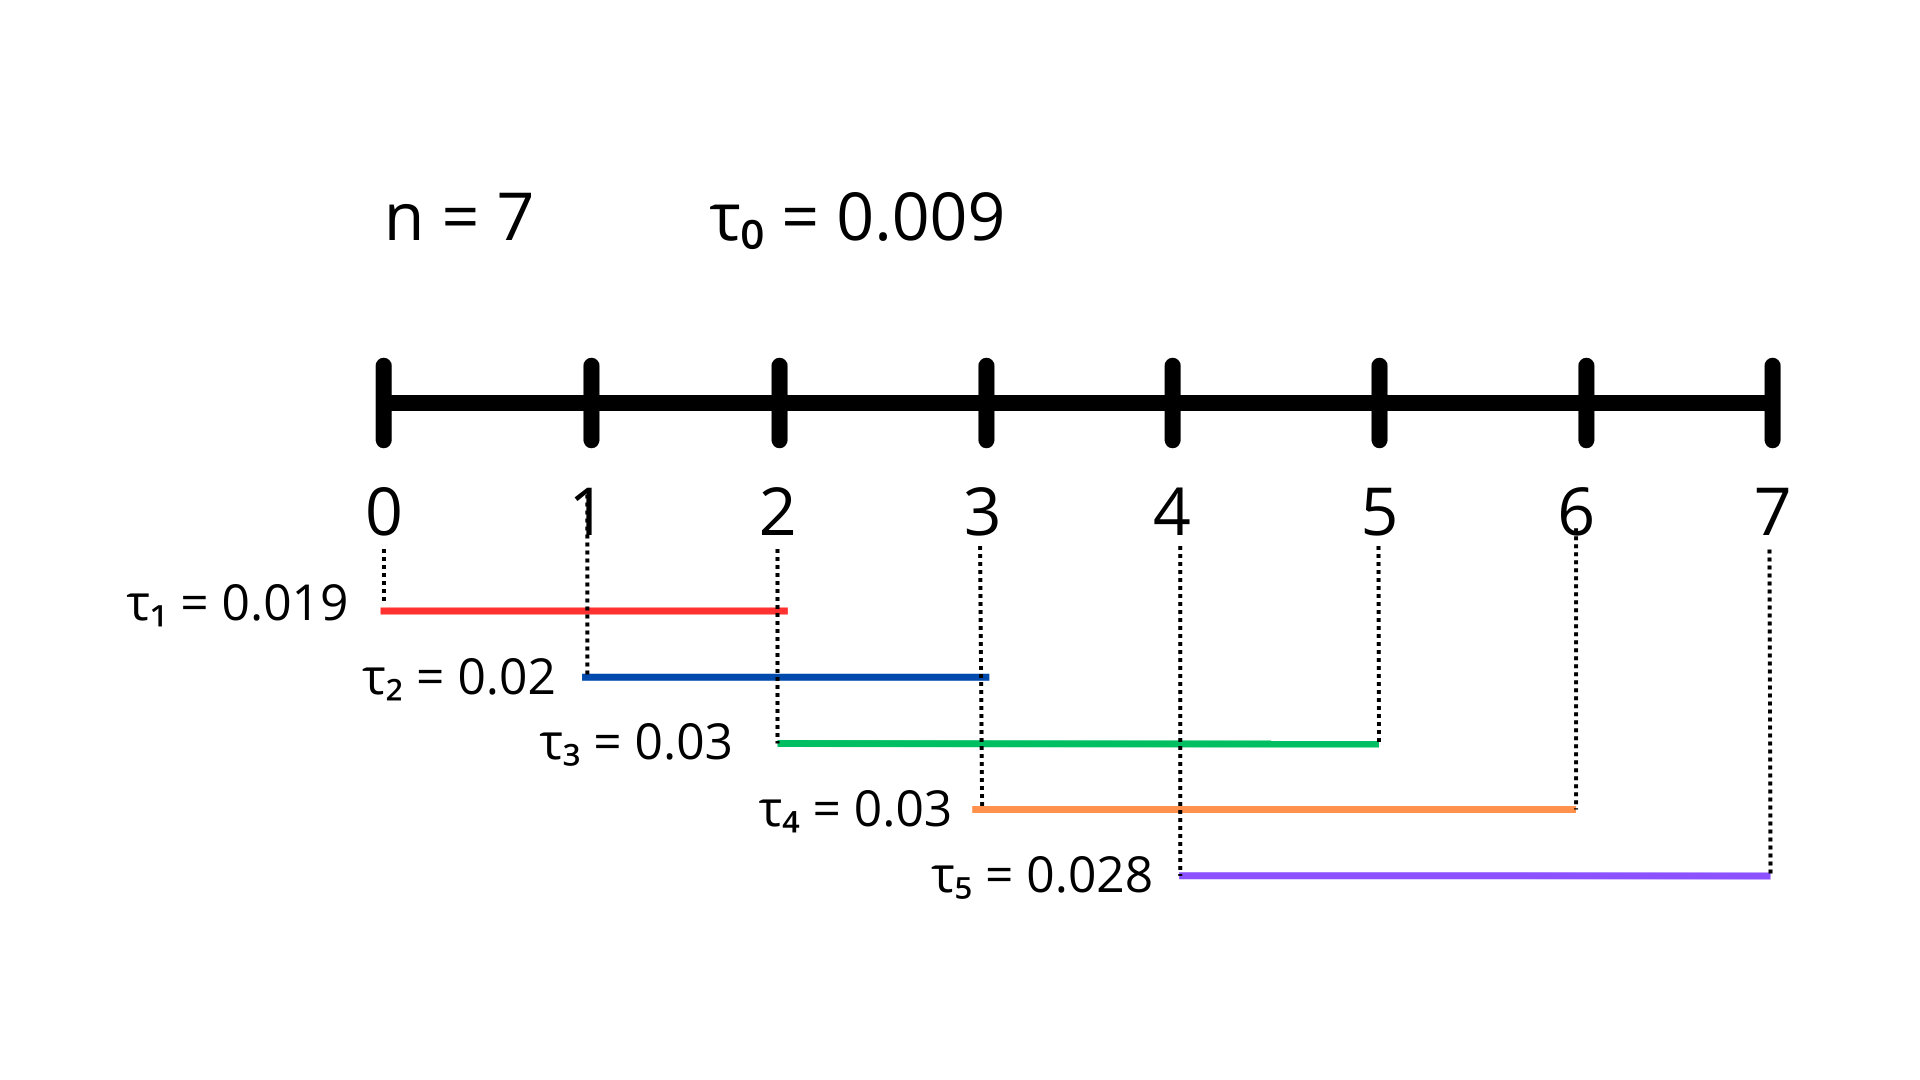
\includegraphics[width=0.85\textwidth]{images/table.png}
	\caption{Table d'orienté $D$ représentant les arcs $(t, t+1)$ et $(d_k, f_k)$ pour l'exemple avec $n = 7$.}
	\label{fig:table_exemple}
\end{figure}

\subsection{Construction du graphe}

On construit un graphe orienté $D = (V, A)$ tel que :
\begin{itemize}
	\item Les sommets $V = \{0, 1, ..., 7\}$ représentent les dates.
	\item Les arcs $(t, t+1)$ avec un taux $1 + \tau_0 = 1.009$ représentent les placements de base.
	\item Les arcs spécifiques $(d_k, f_k)$ avec coefficient $1 + \tau_k$ représentent les produits d’investissement disponibles.
\end{itemize}

Le graphe contient donc :
\begin{itemize}
	\item Arcs de base : (0,1), (1,2), ..., (6,7)
	\item Arcs spécifiques : (0,2), (1,3), (2,5), (3,6), (4,7)
\end{itemize}

\begin{figure}[h!]
	\centering
	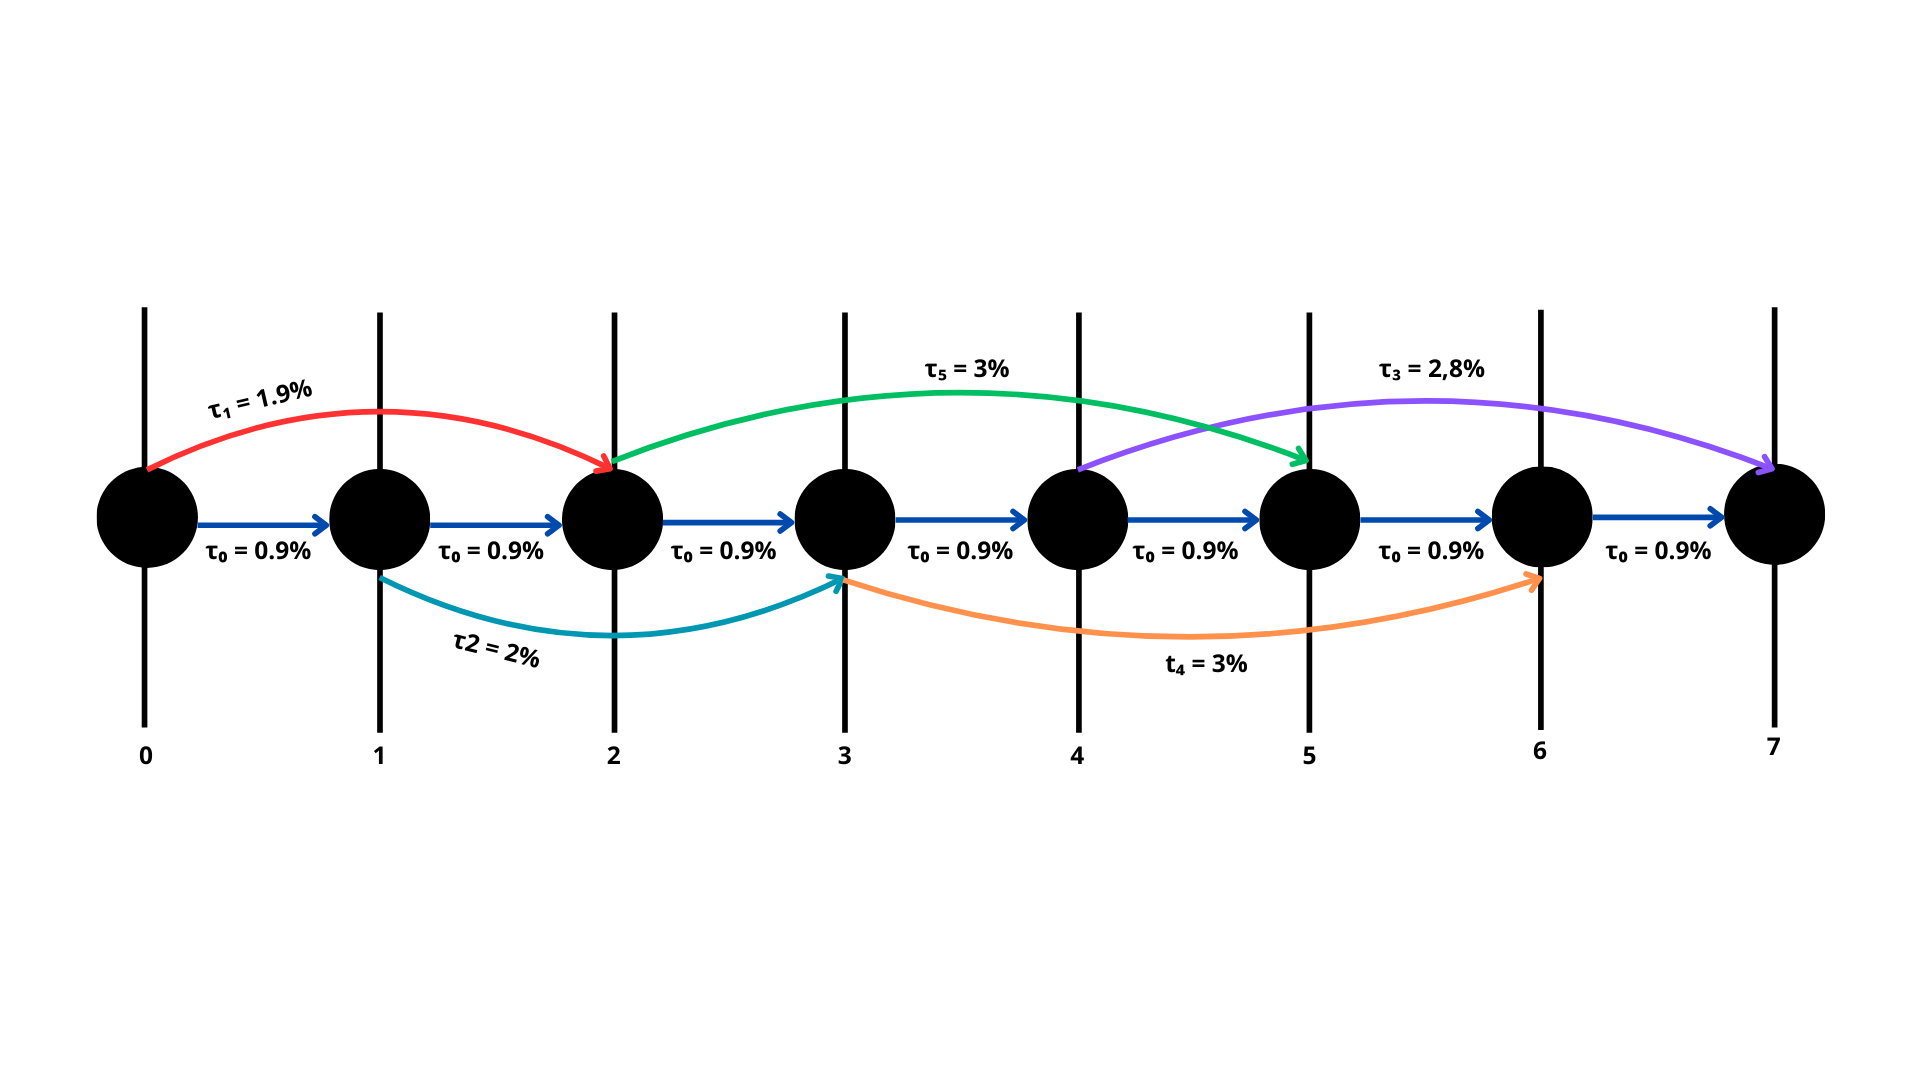
\includegraphics[width=1\textwidth]{images/graph_concret_exemple.png}
	\caption{Graphe orienté $D$ représentant les arcs $(t, t+1)$ et $(d_k, f_k)$ pour l'exemple avec $n = 7$.}
	\label{fig:graphe_exemple}
\end{figure}
\newpage
\subsubsection{Énumération des chemins de P(0, 7).}
Voici une liste des chemins possibles pour aller de la date 0 à la date 7, en ayant utilisé les arcs disponibles, y compris ceux par défaut ("t->t+1") :


\begin{itemize}
	\item Chemin 1 : $(0,1) \to (1,2) \to (2,3) \to (3,4) \to (4,5) \to (5,6) \to (6,7)$ \\
	      \hspace{0.5cm} $\Rightarrow C_1 \approx 1.0647$
	      \vspace{0.3cm}
	      
	\item Chemin 2 : $(0,1) \to (1,2) \to (2,3) \to (3,4) \to (4,7)$ \\
	      \hspace{0.5cm} $\Rightarrow C_2 \approx 1.0655$
	      \vspace{0.3cm}
	      
	\item Chemin 3 : $(0,1) \to (1,2) \to (2,3) \to (3,6) \to (6,7)$ \\
	      \hspace{0.5cm} $\Rightarrow C_3 \approx 1.0676$
	      \vspace{0.3cm}
	      
	\item Chemin 4 : $(0,1) \to (1,2) \to (2,5) \to (5,6) \to (6,7)$ \\
	      \hspace{0.5cm} $\Rightarrow C_4 \approx 1.0676$
	      \vspace{0.3cm}
	      
	\item Chemin 5 : $(0,1) \to (1,3) \to (3,4) \to (4,5) \to (5,6) \to (6,7)$ \\
	      \hspace{0.5cm} $\Rightarrow C_5 \approx 1.0667$
	      \vspace{0.3cm}
	      
	\item Chemin 6 : $(0,1) \to (1,3) \to (3,4) \to (4,7)$ \\
	      \hspace{0.5cm} $\Rightarrow C_6 \approx 1.0675$
	      \vspace{0.3cm}
	      
	\item Chemin 7 : $(0,1) \to (1,3) \to (3,6) \to (6,7)$ \\
	      \hspace{0.5cm} $\Rightarrow \mathbf{C_7 \approx 1.0696}$ \textbf{(chemin optimal)}
	      \vspace{0.3cm}
	      
	\item Chemin 8 : $(0,2) \to (2,3) \to (3,4) \to (4,5) \to (5,6) \to (6,7)$ \\
	      \hspace{0.5cm} $\Rightarrow C_8 \approx 1.0657$
	      \vspace{0.3cm}
	      
	\item Chemin 9 : $(0,2) \to (2,3) \to (3,4) \to (4,7)$ \\
	      \hspace{0.5cm} $\Rightarrow C_9 \approx 1.0665$
	      \vspace{0.3cm}
	      
	\item Chemin 10 : $(0,2) \to (2,3) \to (3,6) \to (6,7)$ \\
	      \hspace{0.5cm} $\Rightarrow C_{10} \approx 1.0685$
	      \vspace{0.3cm}
	      
	\item Chemin 11 : $(0,2) \to (2,5) \to (5,6) \to (6,7)$ \\
	      \hspace{0.5cm} $\Rightarrow C_{11} \approx 1.0685$
	      \vspace{0.3cm}
\end{itemize}

Pour trouver ces routes L'algorithmique de \textit{enumerate\_paths} qui situe en \texttt{utils.py} est utilisé.


\subsection{Cardinalité des chemins pour $n = 7$}
Dans cet exemple, nous avons $n = 7$. Si l'on supposait que le graphe contient tous les arcs possibles $(t', t)$ avec $0 \leq t' < t \leq 7$, alors selon la formule théorique vue précédemment, le nombre total de chemins distincts de $0$ à $7$ serait :
\[
	|\mathcal{P}(0, 7)| = 2^{7 - 1} = 64
\]

Cependant, dans notre cas particulier, seuls certains arcs $(d_k, f_k)$ sont disponibles, en plus des arcs de base $(t, t+1)$. Cela signifie que le graphe est partiellement connecté, et donc le nombre réel de chemins est inférieur à 64.

Une énumération explicite ou une exploration du graphe permettrait de déterminer ce nombre avec précision. Cela justifie encore une fois l’intérêt d’une approche algorithmique dynamique plutôt que l’énumération brute, qui devient rapidement coûteuse.


\subsection{Conclusion sur l’exemple}
Le chemin $(0,2) \to (2,5) \to (5,6) \to (6,7)$ représente une stratégie optimale dans cet exemple. Il combine deux produits à taux élevé (1.9\%, 3.0\%) et termine avec des placements de base. Il permet de maximiser le coefficient multiplicatif total du capital, atteignant environ 1.069 — supérieur à toutes les stratégies fondées uniquement sur le taux de base.

Cet exemple valide la nécessité d’utiliser une approche dynamique pour détecter efficacement la meilleure combinaison.



\section{Recherche de la solution optimale}

\subsection{Pourquoi une approche dynamique ?}

Comme le nombre de chemins possibles de 0 à $n$ peut croître de manière exponentielle, une approche par énumération brute devient rapidement inefficace. Il est donc essentiel d’utiliser une stratégie algorithmique plus performante.  
Nous adoptons une \textbf{programmation dynamique}, qui permet de calculer, de manière itérative, la meilleure valeur atteignable à chaque date $t$ en évitant les répétitions inutiles.

\subsection{Définition de la fonction $Coef(t)$}

Pour chaque date $t \in \{0, 1, ..., n\}$, on définit $Coef(t)$ comme le \textbf{coefficient multiplicatif maximal du capital} que l’on peut obtenir à la date $t$.

Les deux premières valeurs sont connues par hypothèse :
\[
	Coef(0) = 1, \quad Coef(1) = Coef(0) \cdot (1 + \tau_0)
\]

Ensuite, pour chaque $t \geq 2$, la valeur de $Coef(t)$ est calculée récursivement selon la formule suivante :
\[
	Coef(t) = \max \left[
		Coef(t-1) \cdot (1 + \tau_0), \;
		\max_{k \in N^-(t)} \left( Coef(d_k) \cdot (1 + \tau_k) \right)
	\right]
\]

où :

\begin{itemize}
	\item $\tau_0$ est le taux d’intérêt de base par période,
	\item $\tau_k$ est le taux associé au placement spécifique $P_k$,
	\item $d_k$ est la date de début du placement $P_k$,
	\item $f_k$ est la date de fin du placement $P_k$,
	\item $N^-(t)$ est l’ensemble des indices $k$ tels que $f_k = t$ :
	      \[
	      	N^-(t) = \left\{ k \in \{1, 2, ..., m\} \;\middle|\; f_k = t \right\}
	      \]
\end{itemize}





\subsection{Interprétation de la formule}

À chaque instant $t$, deux choix s’offrent à l’investisseur :
\begin{itemize}
	\item continuer avec un placement de base : capital multiplié par $(1 + \tau_0)$,
	\item profiter d’un produit spécifique $P_k$ terminé à la date $t$ : capital multiplié par $(1 + \tau_k)$ à partir de la date $d_k$.
\end{itemize}

La meilleure option est retenue et permet de construire progressivement la valeur optimale $Coef(t)$.

\subsection{Propriété du graphe}

Le graphe $D$ étant orienté et sans cycle (acyclique), on peut traiter les dates dans l’ordre croissant ($t = 0 \to n$), ce qui garantit que chaque $Coef(t)$ peut être construit à partir des valeurs précédentes. Cela assure l’existence d’une solution optimale et rend l’algorithme efficace.

\subsection{Complexité temporelle}

Grâce à l’approche dynamique, la complexité temporelle de l’algorithme est de l’ordre de $\mathcal{O}(n \cdot m)$, où :
\begin{itemize}
	\item $n$ est l’horizon temporel (nombre total de périodes),
	\item $m$ est le nombre de produits financiers spécifiques disponibles.
\end{itemize}

À chaque étape $t$, on ne considère que les $P_k$ tels que $f_k = t$ ; ainsi, le coût est linéaire par rapport à $m$. Cela représente une amélioration significative par rapport à l’énumération exhaustive de tous les chemins, dont la complexité est exponentielle en $n$.

\paragraph{Remarque sur le sens du calcul}

L’algorithme de programmation dynamique progresse dans le sens chronologique : les valeurs $Coef(t)$ sont calculées séquentiellement pour $t = 1$ jusqu’à $t = n$.

Cela est dû au fait que chaque $Coef(t)$ dépend uniquement des valeurs antérieures :
\[
	Coef(t-1) \quad \text{et} \quad Coef(d_k) \quad \text{pour tout } k \text{ tel que } f_k = t
\]
Par conséquent, il est essentiel de connaître toutes les valeurs précédentes avant de pouvoir calculer $Coef(t)$.

En revanche, une fois toutes les valeurs $Coef(t)$ connues, l’extraction du \textbf{meilleur chemin d’investissement} (i.e. la politique optimale) peut se faire en sens inverse, en retraçant les décisions à partir de la date finale $t = n$ jusqu’à $t = 0$.

\section{Implémentation algorithmique}
\subsection{Lecture des données}

L’algorithme commence par lire les données du problème à partir d’un fichier Excel fourni par l’utilisateur.

Le fichier contient :
\begin{itemize}
	\item le nombre total de périodes $n$ ;
	\item le taux d’intérêt de base $\tau_0$ ;
	\item une liste de $m$ produits financiers spécifiques sous forme de triplets $(\tau_k, d_k, f_k)$.
\end{itemize}

Ces données sont extraites et stockées dans trois objets Python :
\begin{itemize}
	\item un entier $n$ : horizon d’étude (nombre d’unités de temps) ;
	\item un flottant $\tau_0$ : taux d’intérêt applicable à chaque intervalle de base $[t, t+1]$ ;
	\item une liste \texttt{placements} contenant les produits $P_k$ sous forme de tuples : \texttt{(tauk, dk, fk)}.
\end{itemize}

La fonction responsable de cette opération est définie comme suit :

\begin{algorithm}[H]
	\caption{Lecture des données depuis un fichier Excel}
	\begin{algorithmic}[1]
		\Function{lecture\_donnees}{fichier}
		\State Lire $n$ et $\tau_0$ depuis la première ligne
		\State Initialiser une liste vide \texttt{placements}
		\For{chaque ligne suivante du fichier}
		\State Lire $(\tau_k, d_k, f_k)$
		\State Ajouter \texttt{(tauk, dk, fk)} à \texttt{placements}
		\EndFor
		\State \Return $(n, \tau_0, \texttt{placements})$
		\EndFunction
	\end{algorithmic}
\end{algorithm}

Cette fonction s’appuie sur la bibliothèque \texttt{openpyxl} pour la lecture du fichier Excel et effectue les conversions nécessaires pour assurer la compatibilité avec les étapes suivantes de l’algorithme.

\vspace{0.5cm}
Un extrait du fichier \texttt{exemple.xlsx} est présenté ci-dessous :

\begin{center}
	\begin{tabular}{|c|c|c|}
		\hline
		$\tau_k$ & $d_k$ & $f_k$ \\
		\hline
		0.019    & 0     & 2     \\
		0.020    & 1     & 3     \\
		0.030    & 2     & 5     \\
		0.030    & 3     & 6     \\
		0.028    & 4     & 7     \\
		\hline
	\end{tabular}
	\captionof{table}{Extrait du fichier \texttt{exemple.xlsx} contenant les produits $P_k$}
	\label{tab:produits-exemple}
\end{center}


\subsection{Calcul du coefficient optimal \texttt{Coef(t)}}

La fonction \texttt{optimiz\_coef} calcule, pour chaque instant $t$, le coefficient multiplicatif maximal \texttt{Coef(t)} que l’on peut atteindre, en choisissant soit de continuer avec le taux d’intérêt de base, soit d’utiliser un placement spécifique qui se termine à $t$.  
En plus, elle enregistre le chemin optimal en stockant dans une liste \texttt{chemin[t]} la date précédente qui a permis d’atteindre cette valeur.

\vspace{0.3cm}

\noindent \textbf{Entrées :}
\begin{itemize}
	\item $t$ : date actuelle.
	\item \texttt{coef} : liste des valeurs déjà calculées pour \texttt{Coef(0)} jusqu’à \texttt{Coef(t-1)}.
	\item $\tau_0$ : taux d’intérêt de base, constant.
	\item \texttt{placements} : liste des placements spécifiques $(\tau_k, d_k, f_k)$.
	\item \texttt{chemin} : tableau où l’on enregistre, pour chaque $t$, la date précédente optimale.
\end{itemize}

\noindent \textbf{Sortie :}
\begin{itemize}
	\item La valeur optimale \texttt{Coef(t)}.
\end{itemize}

\begin{algorithm}[H]
	\caption{Calcul optimal du coefficient \texttt{Coef(t)}}
	\begin{algorithmic}[1]
		\Function{optimiz\_coef}{$t$, \texttt{coef}, $\tau_0$, \texttt{placements}, \texttt{chemin}}
		\State $best \gets \texttt{coef}[t-1] \cdot (1 + \tau_0)$ \Comment{Option de base}
		\State \texttt{chemin}[$t$] $\gets t - 1$ \Comment{On suppose qu’on vient de $t-1$}
		
		\ForAll{$(\tau_k, d_k, f_k)$ dans \texttt{placements}}
		\If{$f_k = t$} \Comment{Placement se terminant à $t$}
		\State $val \gets \texttt{coef}[d_k] \cdot (1 + \tau_k)$
		\If{$val > best$}
		\State $best \gets val$
		\State \texttt{chemin}[$t$] $\gets d_k$ \Comment{On vient de $d_k$ via ce placement}
		\EndIf
		\EndIf
		\EndFor
		
		\State \Return $best$
		\EndFunction
	\end{algorithmic}
\end{algorithm}


\subsection{Reconstruction du chemin optimal}

Après avoir calculé les valeurs optimales \texttt{Coef(t)} pour chaque $t$, on souhaite reconstruire le chemin qui a permis d’atteindre la valeur finale maximale.  
Pour cela, on utilise le tableau \texttt{chemin}, dans lequel chaque case \texttt{chemin[$t$]} indique de quelle date provient la meilleure décision menant à $t$.

La fonction \texttt{reconstruct\_path} suit ce chemin en partant de $t = n$ et en remontant étape par étape jusqu’à $t = 0$, en collectant les couples de transitions $(\texttt{chemin}[t], t)$ qui forment le chemin optimal.

\vspace{0.3cm}

\noindent \textbf{Entrées :}
\begin{itemize}
	\item \texttt{chemin} : liste des antécédents optimaux pour chaque $t$.
	\item $n$ : instant final.
\end{itemize}

\noindent \textbf{Sortie :}
\begin{itemize}
	\item \texttt{path} : liste de transitions optimales sous forme de couples $(t_\text{précédent}, t_\text{actuel})$.
\end{itemize}

\begin{algorithm}[H]
	\caption{Reconstruction du chemin optimal}
	\begin{algorithmic}[1]
		\Function{reconstruct\_path}{\texttt{chemin}, $n$}
		\State $t \gets n$
		\State \texttt{path} $\gets$ liste vide
		
		\While{$t > 0$}
		\State $prev \gets \texttt{chemin}[t]$
		\State Ajouter le couple $(prev, t)$ à \texttt{path}
		\State $t \gets prev$
		\EndWhile
		
		\State Inverser la liste \texttt{path} \Comment{Pour aller de $0$ vers $n$}
		\State \Return \texttt{path}
		\EndFunction
	\end{algorithmic}
\end{algorithm}



\subsection{Programme principal}

Le programme principal permet d’exécuter l’ensemble des étapes de résolution :

\begin{itemize}
	\item Lecture des données à partir d’un fichier Excel (\texttt{lecture\_donnees}).
	\item Initialisation des structures de calcul (\texttt{coef}, \texttt{chemin}).
	\item Calcul des coefficients optimaux $Coef(t)$ par programmation dynamique.
	\item Reconstruction du chemin optimal à partir du tableau \texttt{chemin}.
	\item Affichage du résultat final : valeurs des $Coef(t)$, chemin optimal, et coefficient final.
\end{itemize}

\begin{algorithm}[H]
	\caption{Programme principal d’optimisation}
	\begin{algorithmic}[1]
		\Function{main}{}
		\State Lire les données : $n$, $\tau_0$, \texttt{placements} \Comment{Depuis un fichier Excel}
		\State Initialiser les tableaux \texttt{coef} et \texttt{chemin}
		\State $\texttt{coef}[0] \gets 1$
		\State $\texttt{coef}[1] \gets \texttt{coef}[0] \cdot (1 + \tau_0)$
		\State $\texttt{chemin}[1] \gets 0$
		
		\For{$t$ de 2 à $n$}
		\State $\texttt{coef}[t] \gets \texttt{optimiz\_coef}(t, \texttt{coef}, \tau_0, \texttt{placements}, \texttt{chemin})$
		\EndFor
		
		\State \texttt{path} $\gets$ \texttt{reconstruct\_path}(\texttt{chemin}, $n$)
		
		\State Afficher tous les \texttt{Coef(t)} pour $t = 0$ à $n$
		\State Afficher le chemin optimal \texttt{path}
		\State Afficher \texttt{Coef(n)} comme capital final
		\EndFunction
	\end{algorithmic}
\end{algorithm}


L’exécution du programme sur différentes instances fournit les résultats suivants.

\subsection{Exemple 1 — Données issues du fichier \texttt{exemple.xlsx}}

\subsubsection{Fichier utilisé}

Les données de cette instance sont extraites du fichier :

\begin{center}
	\texttt{data-folder/data-exemple/exemple.xlsx}
\end{center}

\vspace{0.3cm}

\subsubsection{Valeurs optimales du capital}

Voici les coefficients multiplicatifs optimaux $Coef(t)$ calculés pour chaque date $t$ :

\begin{center}
	\begin{tabular}{|c|c|}
		\hline
		$t$ & $Coef(t)$ \\
		\hline
		0   & 1.00000   \\
		1   & 1.00900   \\
		2   & 1.01900   \\
		3   & 1.02918   \\
		4   & 1.03844   \\
		5   & 1.04957   \\
		6   & 1.06006   \\
		7   & 1.06960   \\
		\hline
	\end{tabular}
\end{center}

\vspace{0.4cm}

\subsubsection{Chemin d’investissement optimal}

Le chemin optimal permettant d’atteindre le capital final maximal est le suivant :

\begin{center}
	\texttt{0 $\rightarrow$ 1 $\rightarrow$ 3 $\rightarrow$ 6 $\rightarrow$ 7}
\end{center}

Ce chemin correspond à la stratégie suivante :
\begin{itemize}
	\item placement de base entre $t = 0$ et $t = 1$ ;
	\item produit spécifique $P_2$ utilisé de $t = 1$ à $t = 3$ ;
	\item produit spécifique $P_4$ utilisé de $t = 3$ à $t = 6$ ;
	\item placement de base entre $t = 6$ et $t = 7$.
\end{itemize}

\vspace{0.3cm}

\subsubsection{Capital final obtenu}

Le coefficient multiplicatif total à la fin de la période est :
\[
	\boxed{Coef(7) = 1.06960}
\]

Ce résultat valide la performance de l’algorithme dans l’identification d’une stratégie d’investissement optimale.


\subsection{Exemple 2 — Données issues d’un fichier personnalisé}

\subsubsection{Fichier utilisé}

Les données de cette instance proviennent d’un fichier plus long contenant 129 périodes et un ensemble élargi de produits spécifiques.  
(Nom du fichier non précisé ici — à ajouter si nécessaire.)

\vspace{0.3cm}

\subsubsection{Valeurs optimales du capital}

Voici un extrait des valeurs optimales calculées pour \texttt{Coef(t)} :

\begin{center}
	\begin{tabular}{|c|c||c|c||c|c|}
		\hline
		$t$ & $Coef(t)$ & $t$ & $Coef(t)$ & $t$ & $Coef(t)$ \\
		\hline
		0   & 1.00000   & 20  & 1.23242   & 40  & 1.54233   \\
		60  & 1.92632   & 80  & 2.36578   & 100 & 2.94091   \\
		110 & 3.34756   & 120 & 3.78792   & 128 & 4.22391   \\
		\hline
	\end{tabular}
\end{center}

\vspace{0.4cm}

\subsubsection{Chemin d’investissement optimal}

Le chemin optimal trouvé est relativement long. En voici les principales transitions clés (extrait simplifié) :

\begin{center}
	\begin{tabular}{|c|c|c|}
		\hline
		Étapes               & Transition            \\
		\hline
		0 $\rightarrow$ 4     & Placement spécifique \\ 
		14 $\rightarrow$ 19   & Placement spécifique \\
		34 $\rightarrow$ 54   & Placement spécifique \\
		61 $\rightarrow$ 75   & Placement spécifique \\
		94 $\rightarrow$ 102  & Placement spécifique \\
		102 $\rightarrow$ 107 & Placement spécifique \\
		109 $\rightarrow$ 118 & Placement spécifique \\
		124 $\rightarrow$ 126 & Placement spécifique \\
		126 $\rightarrow$ 128 & Placement final       \\
		\hline
	\end{tabular}
\end{center}

(Toutes les autres transitions intermédiaires sont des placements de base successifs.)

\vspace{0.3cm}

\subsubsection{Capital final obtenu}

Le coefficient final à la date $t = 128$ est :

\[
	\boxed{Coef(128) = 4.22391}
\]

Ce résultat montre que la stratégie optimale sélectionnée par l’algorithme permet de quadrupler le capital initial, en combinant plusieurs placements spécifiques à long terme avec des placements de base réguliers.



\section{Conclusion}

\subsection*{Résumé du Rapport}

Dans ce projet, nous avons étudié un problème d’optimisation de stratégie d’investissement sur un horizon discret donné.  
En modélisant les opportunités de placement sous forme d’un graphe orienté acyclique, nous avons pu appliquer une approche efficace de programmation dynamique permettant de déterminer, à chaque instant $t$, le coefficient multiplicatif optimal du capital.

L’algorithme proposé évite l’énumération exhaustive de tous les chemins possibles (dont le nombre croît exponentiellement) et garantit une solution optimale en temps raisonnable.  
Cette approche est à la fois théoriquement fondée, simple à mettre en œuvre, et très efficace en pratique.


\section*{Annexes}

\subsection*{Installation du module \texttt{openpyxl}}

Pour exécuter correctement le programme Python et lire les données depuis un fichier Excel (.xlsx), il est nécessaire d’installer la bibliothèque \texttt{openpyxl}.

\begin{itemize}
	\item Tapez dans le terminal : \texttt{pip install openpyxl}
\end{itemize}


\end{document}